
\begin{itemize}
\item glitch (because it's important in a space oriented discussion)
\item non linearity. Explain frequency modulation, RF and PF reconstructions
  that may not be strictly linear
\item Explain what we mean by non linearity (ref to previous papers that showed
  the linearity of the KIDs response and that we look at the next order
  correction). Polarized equations with the non linear term.
\item Describe the simulation method : on simule une planete scannee a une
  certaine vitesse, on recalcule le flux etc... pour mesurer la
  non-lin\'earit\'e.
\item Results in RF and PF
\item Application to CMB maps and power spectra estimation
\item HWP associated systematics. The modulation of the HWPSS may bias the
  measurement by inducing non linearity.
\end{itemize}

In view of future utilizations of KIDs in space mission it is necessary to demonstrate the capabilities and the suitability of KIDs arrays in a space like environment. In this section we will adress some of the systematics effects that need to be taken into account during the design of futur generation detector arrays for space applications, such as the KIDs non-linearity.\\

\subsection{Cosmic rays impact on KIDs array}

One of the major problems for space based missions is the impact of an intense flux of high energy particles, referred to as Cosmic Rays (CR) on the detectors. Primary CR are produced by the Sun and by other galactic sources. They are mostly composed by protons (90\%), helium nuclei (9\%) and a few heavier nuclei and electrons (1\%). The CR spectrum is peaked aroud 200 MeV, thus the particles have sufficient energy to penetrate the detectors and give an unwanted signal. The Planck satellite \citep{2014A&A...571A..10P} has demonstrated that the impact of CR on the detectors are a key problem for space missions. Indeed, the glitches caused by CR can mask the real data and induce a loss of an important fraction of it.\\
Experiments have been done to construct a setup that allows to study the behavior of KIDs arrays under typical conditions of a space-borne observatory, and establish the compatibility of KIDs with a space environment \citep{2016A&A...592A..26C,2016SPIE.9914E..0NM}. When the detector is hit by a CR there is a lapse of time during which the sensor is 'blind' to the incoming scientific data. The length of this dead-time depends on the response time of the KID (time constant) which is determined by the quasi particle lifetime. \citet{2012ApPhL.100w2601M} have shown for KID, this time constant is equal to about tens of microseconds which is faster than bolometers (from 5-10 ms to 2s). This means that for the same CR hit, less data is lost when using KIDs arrays. Plus, the experiments have confirmed the fact that KID recover their initial state in less than 5 milliseconds. Finally, \citet{2016SPIE.9914E..0NM} concluded that the percent level of data loss per pixel by a KIDs array placed in a space environment is about 1 \% compared to 15 \% for Planck HFI bolometers.\\ Compared to bolometers, the KID technology shows promising results for compatibility with a space-borne mission, as their extremely short glitch time constant permits to greatly reduce the data loss fraction due to CR impacts. 

\subsection{KIDs non-linearity}

One of the key systematic effect that we must take into account is the KID non-linearity induced by the detector and the method we use to reconstruct the absorbed signal. In this paper, we will focus on the KID non linearity and how it impacts on a measurement of the CMB polarization.\\

The KIDs linearity has been demonstrated, over a large power range, in laboratory under realistic conditions as shown in Fig. \ref{KID-lin}. As we can see, at 300K the response of the KID is still under a linear regime.

\begin{figure}[h]
\center
	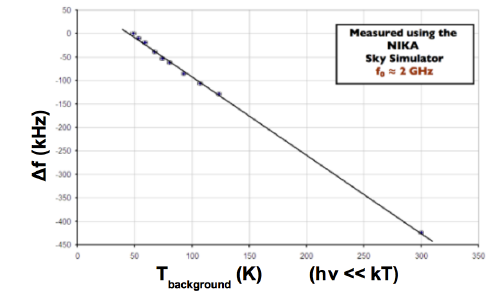
\includegraphics[scale=0.4]{KID-linearity-Monfardini2014.png}
	\caption{KID linarity demonstrated in laboratory under realistic conditions. Y-axis : frequency shift of the resonance (KID measured signal), X-axis : optical background temperature. The solid line represents the linear fit of the experimental points. Credits : \citet{2014JLTP..176..787M}.}
	\label{KID-lin}
\end{figure}

In this section we look at the next order correction, meaning that we will focus on the non-linear term produced by the detector and the way that we reconstruct the signal. A measure done by the KID is defined by $m = T + P$, with $T$ and $P$ representing the temperature and polarization. The non-linearity is characterized  by the $\varepsilon$ coefficient in $ m = m_{1} + \varepsilon m_{1}^{2}$. We have : 

\begin{equation}
\begin{split}
m & = m_{1} +\varepsilon' (T+P)^{2} \\
 & = T + P + \varepsilon'(T^{2} + P^{2} + 2TP) 
\end{split}
\end{equation}

Therefore, knowing that $T=I$ and $P = Q\cos(2\alpha) + U \sin(2\alpha)$, the polarized equation with a non-linear term is given Eq. \ref{eq-NL}.

\begin{equation}
m  \simeq (I + \varepsilon' I^{2}) + (Q + 2\varepsilon' IQ) \cos(2\alpha) + (U + 2 \varepsilon' IU) \sin(2\alpha)
\label{eq-NL}
\end{equation}

The non-linear coefficient is induced by the detector and the method used to reconstruct the signal. These methods are described in the following section.

\subsection{Methods of signal reconstruction}
\subsubsection{Modulated readout technique}
One of the most difficult challenges of operationg a KID compared to a bolometer is to convert the $I(t)$ and $Q(t)$ values to an absorbed optical power or shift in resonant frequency as a function of time $\delta f_{0} \propto \delta P_{opt}$. To address this problem, an innovative readout technique has been developed to monitor the change of the signal $\frac{dI}{df}$,$\frac{dQ}{df}$ by using a known frequency shift. This scheme allows continuous simultaneous tracking of KID resonant frequency which change proportionally to the absorbed optical power. To do so, the standart excitation of the detectors which uses a fixed tone is replaced by a new excitation based on two different frequencies. In fact, in order to generate two tones, we modulate the local oscillator signal between two values, separated by $\delta f_{LO} \simeq 1$ kHz, and obtain $f_{+} = f_{0} + \frac{\delta f_{LO}}{2}$ and $f_{-} = f_{0} - \frac{\delta f_{LO}}{2}$ with $f_{0}$ the detector resonant frequency.\\
The values ($I(t)$,$Q(t)$) are then given by :

\begin{equation}
(I(t),Q(t)) = (\frac{I(f_{+}) + I(f_{-})}{2}, \frac{Q(f_{+}) + Q(f_{-})}{2})
\end{equation}

and the differential values are :

\begin{equation}
\label{gradient}
(\frac{dI}{df}(t),\frac{dQ}{df}(t)) = (\frac{I(f_{+}) - I(f_{-})}{\delta f_{LO}}, \frac{Q(f_{+}) - Q(f_{-})}{\delta f_{LO}})
\end{equation}

\begin{figure}[h]
\center
	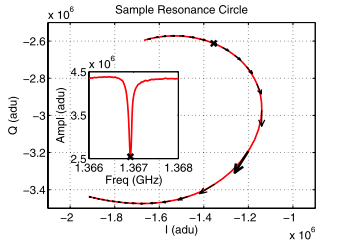
\includegraphics[scale=0.5]{resonance-circle.png}
	\caption{Representation in the I-Q plane of a sweep around a resonance. The red line represents the $(I,Q)$ data of the frequency sweep around the resonance.The arrows reprsents ($\frac{dI}{df}$,$\frac{dQ}{df}$). \citep{2013A&A...551L..12C}}
	\label{circle-iq}
\end{figure}

Fig. \ref{circle-iq} shows a typical KID resonance circle. Thanks to this modulation technique, we obtain four quantities : I, Q and their variation $\delta I$, $\delta Q$.\\
In this paper, I(t) and Q(t) are sampled at 22 Hz, they are the mean values of sub-sample i(t) and q(t) on $N_{m}$ = 40 points at 880 Hz. dI(t) and dQ(t) are the mean values of the difference between the data measured at $f_{-}$ and $f_{+}$. Then we have :

\begin{equation}
I = \sum^{N_{m}=40}_{p=1} i_{p}
\end{equation}

\begin{equation}
Q = \sum^{N_{m}=40}_{p=1} q_{p}
\end{equation}

\begin{equation}
dI = \sum^{N_{m}/2=20}_{p=1} i_{2p} - i_{2p-1}
\end{equation}

\begin{equation}
dQ = \sum^{N_{m}/2=20}_{p=1} q_{2p} - q_{2p-1}
\end{equation}

As shown in the next paragraph, these quantities are used to reconstruct the resonance frequency and so the optical power absorbed by the detector.

\subsubsection{RfdIdQ}
To reconstruct the signal absorbed by the detector, a method was developed named RfdIdQ.\\
If a variation $\Delta I(t)$, $\Delta Q(t)$ is observed between successive  ($I(t)$, $Q(t)$) points, it is possible to estimate the value of $\delta f_{0}$ by comparing ($\Delta I(t)$, $\Delta Q(t)$) with the gradient $(\frac{dI}{df}(t),\frac{dQ}{df}(t)) $. This is done by projecting ($\Delta I(t)$, $\Delta Q(t)$) along the gradient found in Eq.\ref{gradient}. The shift of the resonant frequency between two samples is then determined with Eq.\ref{Rf} \citep{2014A&A...569A...9C}

\begin{equation}
\label{Rf}
\Delta (\delta f_{0}(t)) = \delta f_{LO} \frac{\Delta I<dI>_{50} + \Delta Q<dQ>_{50} }{<dI>_{50}^{2} + <dQ>_{50}^{2}}
\end{equation}

\begin{equation}
\delta f_{0}(t) = \sum^{t}_{t'=0} (\Delta (\delta f_{0})(t'))
\end{equation}

\footnote{$<.>_{50}$ means that we average the considered quantities over 50 points before and after the concerned value.}

This method is convenient, but can be affected by some systematic uncertainty and be a source of non-linearity. In fact, $(\frac{dI}{df}(t),\frac{dQ}{df}(t))$ is tangeant to the (I,Q) circle for a fixed background optical power, whereas the actual variation ($\Delta I$, $\Delta Q$) (occurs for a fixed excitation frequency and is due to a difference in the optical power, wich includes a change in the (I,Q) circle radius.). As a consequence, the observed (I,Q) trajectory is not precisely parallel to the direction given by $(\frac{dI}{df}(t),\frac{dQ}{df}(t))$. The predicted error induced by the projection method is less than 2\% for faint sources \citep{2013A&A...551L..12C}. In addition, by averaging $dI$ and $dQ$ we apply a $dI$,$dQ$ that can be very different from reality, in particular when we are near the resonance, with a bright source.\\

\subsubsection{Cf}
To compensate for the errors brought by the rfdidq method, we developed a new technique named Cf (circle fit).\\
The idea of this method is to project I, Q, dI, dQ, onto an axis $y_{3}$ which is as linear as possible with frequency, and so is assumed to be linear with the optical power. In fact, we suppose that :

\begin{equation}
\label{hyp-f}
f = f_{0} + \frac{w}{2} tan\frac{\phi}{2}
\end{equation}

We know that when near a resonance $Z = I+jQ$ is on a circle. To construct $y_{3}$ we scale, translate, rotate and inverse the initial circle to transform it into an infinite radius circle described by :

\begin{equation}
\label{Zres}
Z_{res} = 1 - i tan\frac{\varphi}{2}
\end{equation}

According to Eq. \ref{hyp-f}, the imaginary part of $Z_{res}$ is linearly dependant with the frequency and so represents $y_{3}$, $y_{3} \propto f - f_{0}$.\\
Here to calibrate this dependency and reconstruct the signal, we use I, Q, dI and dQ measurements. By applying the transformations, I, Q, dI and dQ become : 

\begin{equation}
I_{res} = - \frac{1}{2r}[(I-x_{c})cos\alpha + (Q - y_{c})sin \alpha] + \frac{1}{2}
\end{equation}
\begin{equation}
 Q_{res} = \frac{1}{2r}[-(I-x_{c})sin\alpha + (Q - y_{c})cos \alpha] 
\end{equation}

\begin{equation}
dI_{res} = -\frac{1}{2r}(dI cos\alpha + dQ sin\alpha)
\end{equation}

\begin{equation}
dQ_{res} = \frac{1}{2r}(-dI sin\alpha + dQ cos\alpha)
\end{equation}

with : ($x_{c}, y_{c}$), r and $\alpha$ respectively, the center, radius and rotation angle of the initial circle.\\
Then, $dy_{3} = Im(dZ_{res})$. According to the hypothesis in Eq. \ref{hyp-f}, f is a polynom, so to reconstruct the shift in the resonant frequency we can easily fit $\frac{\Delta f}{dy_{3}}$ by a polynomial function and integrate it to obtain the relative frequency of the KID.

%In the next section we describe an innovative modulated readout schemewhich enables the opti- cal power absorbed by a KID to be continuously monitored and leads to a large improvement in the consistency of the photomet- ric calibration.

\subsection{Simulations}
To adress the KIDs non-linearity, we need to measure its non-linearity coefficient $\varepsilon$ by doing simulations of the KID response to an incoming source of radiation, using the Rfdidq and Cf methods.

	\subsubsection{Method}
The simulation method consists first in modelling a scan of planet with a more or less important flux, at a certain speed. Then we recalculate the incoming flux thanks to the modulation technique and the rf/cf method. Finally, we stock the outcoming flux to be able to deduce the non-linearity coefficient.

	\subsubsection{Results}


\section{Application to CMB maps and power spectra estimations}
\section{HWP associated systematics}